\documentclass[11pt,a4paper]{article}
\usepackage[utf8]{inputenc}
\usepackage{amsmath}
\usepackage{amsfonts}
\usepackage{amssymb}
\usepackage{graphicx}
\usepackage{tikz}
\usepackage{multirow}
\usepackage{rotating}
\usetikzlibrary{positioning}
\author{Bastiaan Weijers \\ 3256669 \and Colin Smits \\ 4075390}
\title{Evaluation of a Body Photo Browser}
\begin{document}
\maketitle
\abstract{Here comes the abstract}\\
\textbf{keywords:}
 
\noindent\makebox[\linewidth]{\rule{\textwidth}{0.4pt}}
\section{Introduction}
\section{System Evaluation}
In this chapter we will discuss how the system evaluation was performed and what the results were of this evaluation. 
\subsection{Methods and Environment}
To quantify the performance of the Body Motion program, we setup a test environment to measure how well the system can translate user interaction to concrete system actions. The test setup is contained in an ecologically sound environment, in this case a bedroom with closed curtains was used with as a primary light source three led bulbs lighting the room. There was a single participant used to create quantifying data, whereas the particular user was well introduced to the workings, capabilities and limitations of the system. An analysis of how the system performs when used by lesser informed participants can be found later on in Section 3 - User Evaluation.
\\ The software was used with a YCrCb spectrum at [..   ...] and a minimum delay of $70ms$ between actions, further settings were left at program-default.
\\ For each action performed in the video recording, a chart was updated with the value the system interpreted it to be. Possible predicted and actual actions were: Next, Previous, CW rotation, CCW rotation and Nothing. Whereas "Nothing" is represented as an idle action wherein nothing happens. It is worth noting that this particular action can only be actively observed on the actual outputs of the system, as predicting idle actions is not possible in our system.
\subsection{results}
To achieve accurate and representing results, we have recorded a total of 159 actions that we will measure its interpretation by system off, this accounts to roughly 40 actions per possible move.  The number was picked as such because a $n > 30$ will give us a normal distribution over our data [ref needed]. All actions are recorded in a total of two video's, this allows the system to run in a continuous mode, without having to reinitialize after every action. This continuous mode should yield results that are more ecologically sound as opposed to having system global variables reinitialized with every action.
\\ The evaluated output of a the actions will be tested against their expected outputs, the result of this can be found in Table~\ref{table:systemeval}. The data from the table shows the Predicted actions against the Actual actions delivered by the system for every possible action. From the table one can read how many predictions actually translated to correct behavior of the system, and how many did something unexpected.
\\ Table~\ref{table:systemeval} can be parsed to a so-called Confusion Matrix, which is depicted in Table~\ref{table:confusionmatrix}. This matrix is a further generalization and will help us in the question on how well our system performs. Stated before (????, dit is wel in de presentatie gezegd maar nemen we 't op in de paper?), a preferred bias exists in having low false positives as this might be experienced by end-users as undesired behavior. From looking at the Confusion matrix we strongly suspect that we have satisfied this condition, but to confirm this we need to look at the Precision and Recall and establish a PR-curve.
\\ hier een stuk over precision, recall en pr-curve.
\\ moeten we nog een H0 opstellen voor de confusion matrix? We kunnen misschien proeven dat false positive < false negative?
\\ Verder zien we uit Tabel 1 al dat de PR-curve voor swift-left/right er heel anders uit zal zien dan de PR-curve voor rotation. Die laatste is gewoon beroerd, terwijl de precision en recall voor left/right vrij goed zullen zijn. Dit apart testen denk ik in een subhypothese?

\begin{table}
\begin{center}
\begin{tabular}{|c|c|c|c|c|c|c|}
\cline{3-7}
\multicolumn{2}{c|}{} & \multicolumn{5}{c|}{Predicted action} \\
\cline{3-7}
\multicolumn{2}{c|}{} & Next & Previous & CW & CCW & Nothing \\
\hline
\multirow{6}{*}{\begin{sideways} Actual action ~ \end{sideways}} & Next & 34 & 0 & 0 & 0 & 0 \\
\cline{2-7}
& Previous & 1 & 32 & 0 & 0 & 2 \\
\cline{2-7}
& CW & 0 & 0  & 22  & 4  & 6  \\
\cline{2-7}
& CCW  & 0  & 0  & 0  & 14 & 0  \\
\cline{2-7}
& Nothing & 2 & 5  & 16  & 21  & 0  \\
\hline
\end{tabular}
\end{center}
\caption{Testresults System Evaluation, $n=159$}
\label{table:systemeval}
\end{table}

\par
The data as presented can be further parsed into a confusion matrix which is shown in Table~\ref{table:confusionmatrix}.



\begin{table}
\begin{center}
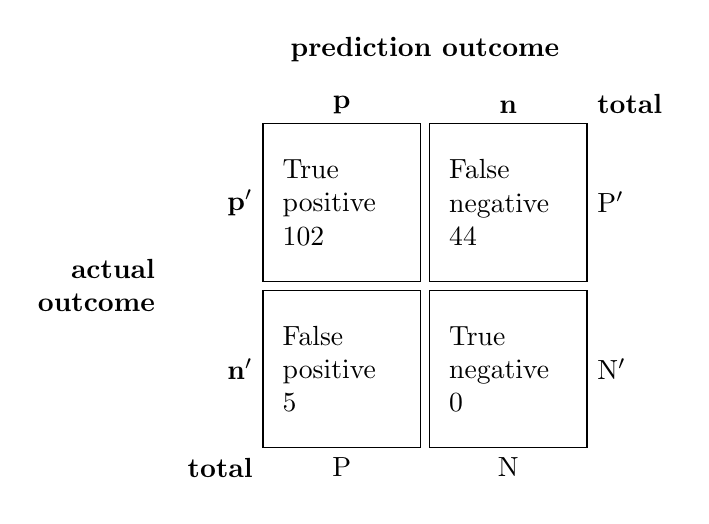
\begin{tikzpicture}[
box/.style={draw,rectangle,minimum size=2cm,text width=1.5cm,align=left}]
\matrix (conmat) [row sep=.1cm,column sep=.1cm] {
\node (tpos) [box,
    label=left:\( \mathbf{p'} \),
    label=above:\( \mathbf{p} \),
    ] {True \\ positive \\ 102};
&
\node (fneg) [box,
    label=above:\textbf{n},
    label=above right:\textbf{total},
    label=right:\( \mathrm{P}' \)] {False \\ negative \\ 44};
\\
\node (fpos) [box,
    label=left:\( \mathbf{n'} \),
    label=below left:\textbf{total},
    label=below:P] {False \\ positive \\ 5 };
&
\node (tneg) [box,
    label=right:\( \mathrm{N}' \),
    label=below:N] {True \\ negative \\ 0};
\\
};
\node [left=.05cm of conmat,text width=1.5cm,align=right] {\textbf{actual \\ outcome}};
\node [above=.05cm of conmat] {\textbf{prediction outcome}};

\end{tikzpicture}
\end{center}
\label{table:confusionmatrix}
\caption{Confusion Matrix}
\end{table}

\subsection{Discussion}
Hier discussie over de resultaten. Hoewel de resultaten nog ontbreken, weten we waarschijnlijk al wel waar de resultation heengaan. Overall scores zullen 'mediocre' zijn at-best. Tenzij we de hypotheses opsplitsen en apart kijken naar swipe-left/right en rotatie. Dan kunnen we misschien iets zeggen over het verschil daarin. We kunnen dan ook "recommendations" maken.








\section{User Evaluation}
\section{Discussion}

\thebibliography{99}

\end{document}